\chapter*{Multiple Target Tracking in World Coordinate with single Camera}
\section{Introduction}
Tracking multiple objects is critical task in many application domains, such as surveillance, autonomous vehicle and robotics. In many of these applications it is desirable to detect moving humans or other targets as well as identify their spatial-temporal trajectories. Such information can enable the design of activity recognition systems for interpreting complex behaviors of individuals and their interaction with the environment.\\ 
This can also provide crucial information to help an autonomous system to explore and interact with complex environments.
Challenging tasks of tracking system can be identified in:
\begin{itemize}
\item estimate stable and accurate tracks and uniquely associate them to a specific object; \item associate tracks to 2D/3D-temporal trajectories in the 3D scene; 
\item work with the minimal hardware equipment (e.g., single
camera-vs-stereo cameras; no laser data); 
\item work with a moving camera. 
\end{itemize}
Meeting all these desiderata is extremely difficult. For instance estimating stable
tracks is difficult as objects are often subject to occlusions (they cross each other
in the image plane), illumination conditions can change in time, the camera mo-
tion can disturb the tracking procedure. Estimating tracks (trajectories) in the
3D world (or camera) reference system is also very hard as estimating 3D world-2D image mapping is intrinsically ambiguous if only one camera is available and
camera parameters are unknown. Structure from motion (SFM) techniques are
often inadequate to estimate motion parameters because the reconstruction is
noisy and unreliable if small baseline is considered. Another problem arise with cluttered dynamic scenes where moving elements violate the SFM assumption of static background.
Another limitation of SFM is that it is computationally expensive and can be hardly implemented in real time.
Inspired by the work of [1] wherein a method for integrating multiple cues
(such as odometry, depth estimation, and object detection) into a cognitive feed-
back loop was proposed, we present a new framework for tackling most of the
issues introduced above in a coherent probabilistic framework. Specifically, our
goals are to: 
\begin{itemize}
\item solve the multi-object tracking problem by using a single uncalibrated moving camera; 
\item handle complex scenes where multiple pedestrians are moving at the same time and occluding each other; 
\item estimate the 2D/3D temporal trajectories within the camera reference system.
\end{itemize}
The key contribution of our work relies on the fact that we simultaneously estimate the camera parameters (such as focal length and camera pose) and track objects (such as pedestrians) as they move in the scene. 
Tracks provide cues for estimating camera parameters by using their scale and velocity in the image plane; at the same time, camera parameters can help track objects more
robustly as critical prior information becomes available. This, in turn, allows
us to estimate object 3D trajectories in the camera reference system. Inspired
by [2], we utilize a simplified camera model that allows to find a compact (but
powerful) relationship between the variables (targets and camera parameters) via
camera projection constraints. The identification of a handful of feature tracks
associated with the static background allows us to add additional constraints to
the camera model. Eventually, we frame our problem as a maximum-posterior
problem in the joint variable space. In order to reduce the (otherwise extremely)
large search space caused by the high dimensionality of the representation, we
incorporate MCMC particle filtering algorithm which finds the best explanation
in sequential fashion. Notice that, unlike previous methods using MCMC, our
method is the first that uses MCMC for efficiently solving the joint camera
estimation and multi-target problem.
The second key contribution is that we obtain robust and stable tracking
results (i.e. uniquely associate object identities to each track) by incorporating
interaction models. Interaction between targets have been largely ignored in the
object tracking literature, due to the high complexity in modeling moving targets
and the consequential computational complexity. The independent assumption
is reasonable when the scene is sparse (only few objects exists in the scene). In a
crowded scene, however, the independent motion model often fails to account for
the target’s deviation from the prediction, e.g. if a collision is expected, targets
will change their velocity and direction rapidly so as to avoid a collision. Thus,
modeling interactions allows us to disambiguate occlusions between targets and
better associate object labels to underlying trajectories. This capability is further
enhanced by the fact that our trajectories are estimated in 3D rather than in the
image plane. Our interaction models are coherently integrated in the graphical
model introduced above.

\section{ Multi-Tracking Formulation problem}\label{sec: MultiTracking Model}
Given a video sequence, our goal is to jointly:
\begin{itemize}
\item track multiple moving or static targets (e.g. cars, pedestrians), 
\item identify their trajectories in 3D with respect to the camera reference system
\item estimate camera parameters (focal length, viewing
angle, etc). 
\end{itemize}
We model each target as a hidden variable $Z_i$ in 3D space whose trajectory in time must be estimated and separated from all other trajectories.
Estimating trajectories in 3D is more robust than estimating trajectories in the image plane because we can impose a number of priors in actual 3D space as we shall see next.
Such trajectories in 3D are estimated by measuring their projections onto 2D image plane which represent our observation variables $X_i$.
Observation $X_i$ is described as $5\times1$ vector containing the center $C(u,v)$ of bounding box enclosing the detected object on image,its dimensions $w \times h$ and the scale $s$ at which the object detector has the found the best matching with object model.
Given the observations $X_i$ found by object detector, tracks $Z_i$ in 3D are estimated by jointly searching the most plausible explanation for both camera and all the existing targets’ states using the projection function $f_P$ characterizing by the camera model.\\
\subsection{Camera Model}
A 3D Target  $Z= [x_z, z_z, h_z]$ in world coordinate system, is characterized by it's projection on ground plane $(x_z, z_z)$ and its height $h_z$ and is related to its location $\hat{Z}$ in the camera coordinate system through the relation \ref{eqn: Exstrinsic Transform}, as depicted in figure
\begin{eqnarray} \label{eqn: Exstrinsic Transform}
Z= \left[ 
\begin{array}{cc}
R(\phi_{\theta} ) & 0 \\
0 & 1
\end{array} 
\right] \hat{Z} +
\left[ 
\begin{array}{c}
x_{\theta} \\
z_{\theta}
\end{array}
\right]
\end{eqnarray}
where:
\begin{itemize}
\item $R(\phi_{\theta})$ is the $2\times2$ rotation matrix encoding the panning of the camera (rotation around $h$ axis) with angle specified by $\phi_{\theta}$ .
\item $x_{\theta}$, $z_{\theta}$ are the 3D location respect to reference system associated to the initial frame.
\end{itemize}
The Camera Extrinsic Parameters are encoded by $3\times1$ parameters vector $Ce_{\theta}=\{\phi_{\theta}, x_{\theta}, z_{\theta}\}$ encoding the rigid transformation depicted in figure \ref{fig: Estrinseci}
\begin{figure}\label{fig: Estrinseci}
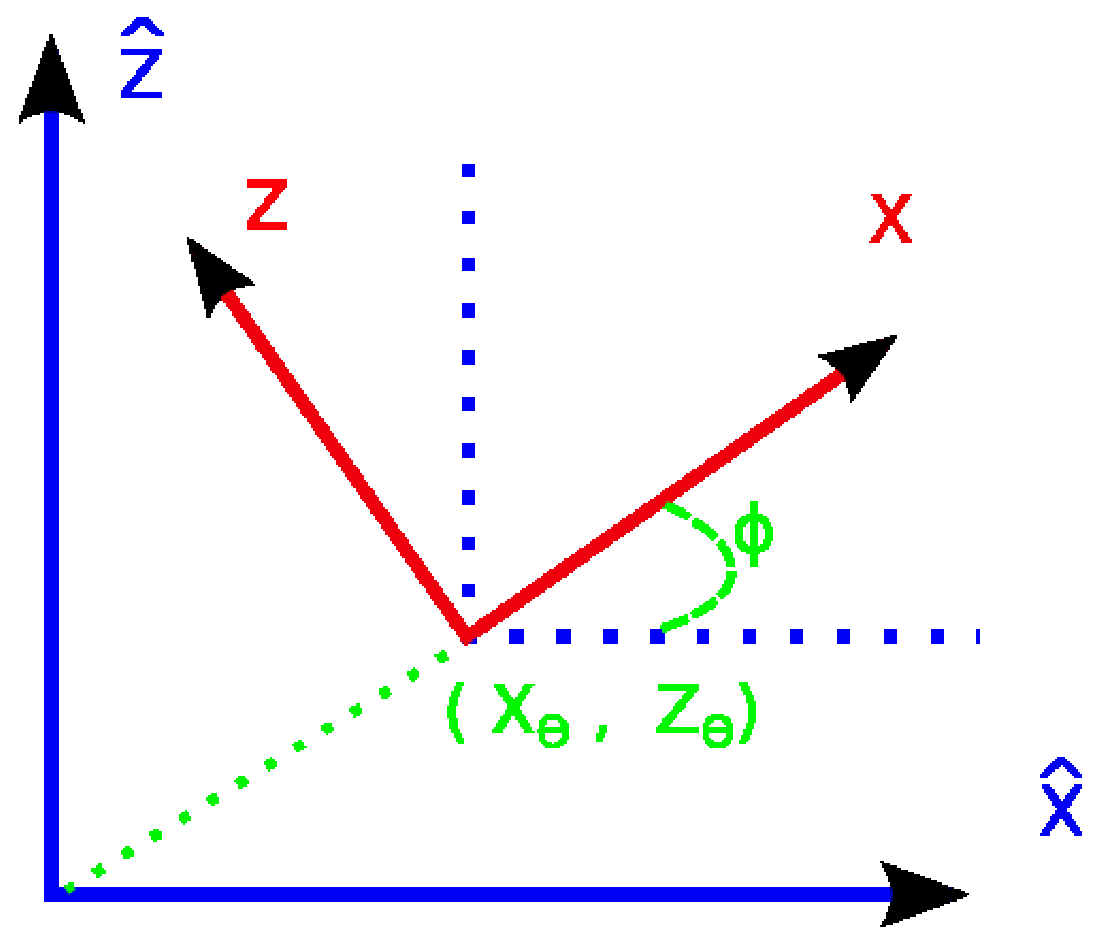
\includegraphics[width=0.5\textwidth]{ImaginiLatex/Estrinseci.eps} 
\caption{ Camera Extrinsic Parameters encoding the rigid transform between camera coordinate system and world coordinate system}
\end{figure}
The camera is supposed to be at random height $h_{\theta}$,  moving with absolute velocity $r_{\theta}$ with the $Z_cam$ axis aligned with the Optic Axis and the $Y_cam$ axis pointed to the ground plane as depicted in figure \ref{fig: UV}.
\begin{figure} \label{fig: UV}
\begin{tabular}{cc} 
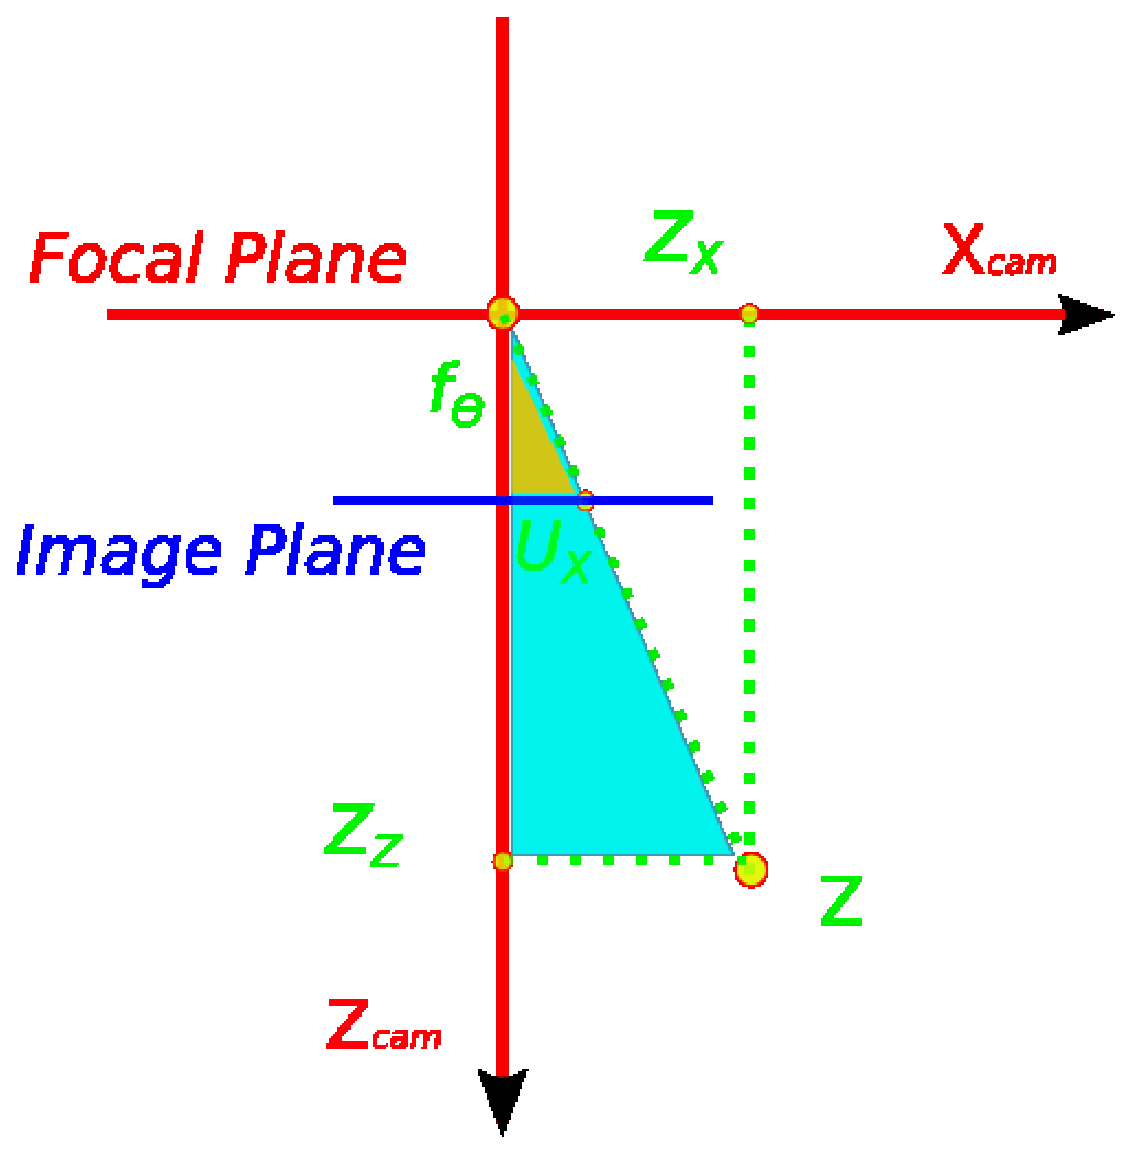
\includegraphics[width=0.5 \textwidth]{ImaginiLatex/Ux.eps} &
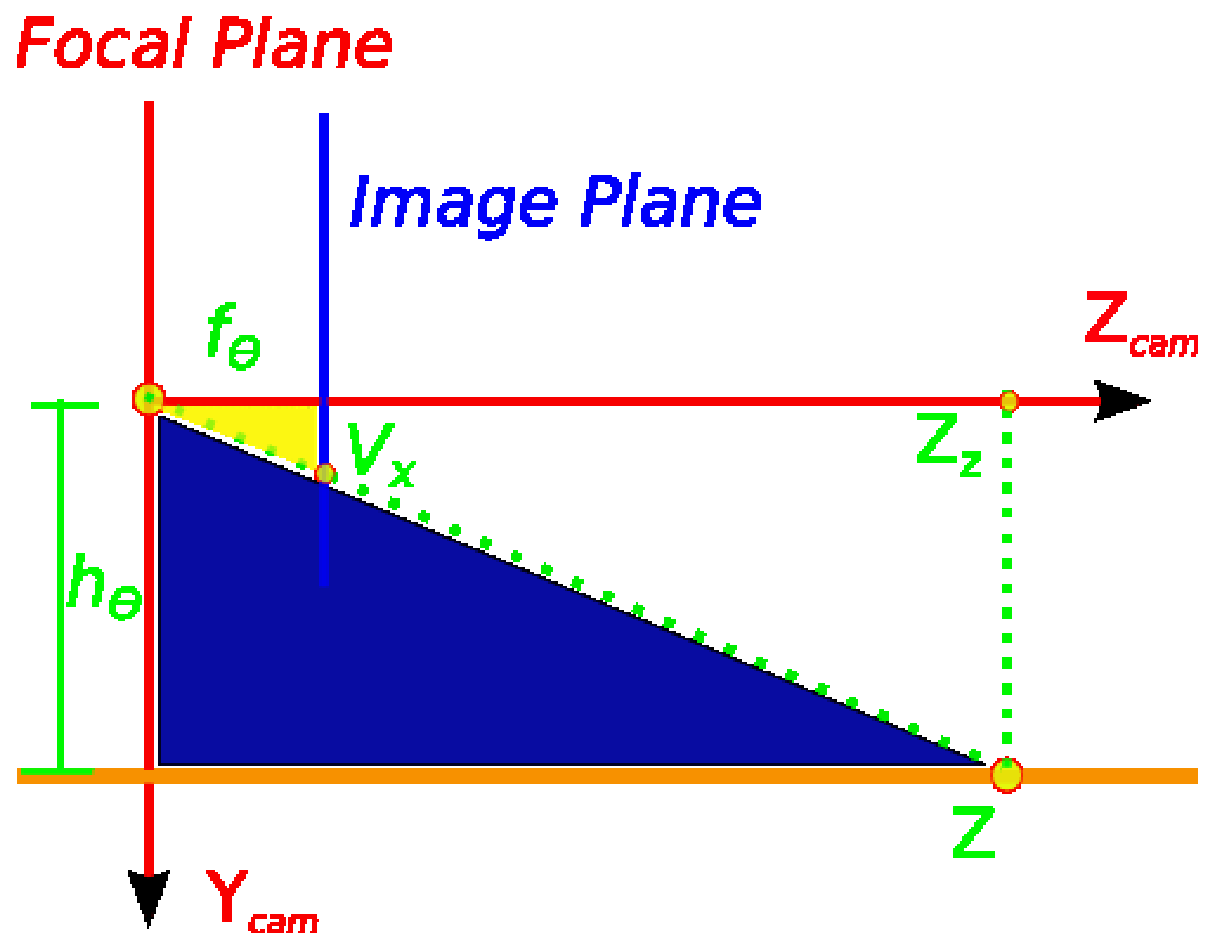
\includegraphics[width=0.5\textwidth]{ImaginiLatex/Vx.eps} \\
\textbf{a} & \textbf{b}
\end{tabular}
\caption{\textbf{a} Since the yellow and the azure triangle are similar,the equality $f_{\theta}:z_z = u_X:x_z$ holds. \textbf{b} Since the yellow and the blue triangle are similar, the equality $f_{\theta}:z_z = v_X:h_{\theta}$ holds. }
\end{figure}

Each 3D Object $Z$ is then projected on the image plane trough the equation: 
\begin{eqnarray} \label{eqn: Perspective Projection}
X=f_P(Z,\Theta)= \left[
\begin{array}{c}
u_X \\
v_X\\
h_X
\end{array}
\right]
= \left[
\begin{array}{c}
\frac{f_{\theta} x_z}{z_z} +u_{\theta} \\
\frac{f_{\theta} h_{\theta}}{z_z} +v_{\theta} \\
\frac{f_{\theta} h_z}{z_z}
\end{array}
\right]
\end{eqnarray}
where:
\begin{itemize}
\item $(u_X,v_X)$ are the bottom-center point location of the 3D Object,
\item $h_X$ is the Height of the 3D Object measured in the image,
\item $f_{\theta}$ is the focal length,
\item $u_{\theta}$ horizontal center point,
\item $v_{\theta}$ horizon position.
\end{itemize}
The Camera Intrinsic parameters are collected in the $4\times1$
$Ci_{\theta}=\{ f_{\theta}, u_{\theta}, v_{\theta}, h_{\theta} \}$ .\\
The Inverse projective transform is given by:
\begin{eqnarray} \label{eqn: Inverse Perspective Projection}
\hat{Z} = f_P^{-1}(X,\Theta)=
 \left[
\begin{array}{c}
\frac{ h_{\theta} (u_x-u_{\theta}) }{ v_x-v_{\theta}} \\
\frac{ f_{\theta} h_{\theta} }{v_x-v_{\theta}} \\
\frac{ h_{\theta} h_z}{v_x-v_{\theta}}
\end{array}
\right]
\end{eqnarray}
The final Hidden Variable describing the Camera Model is then characterized by the
$8\times1$ vector $\Theta=\{ Ci_{\theta},Ce_{\theta},r_{\theta}\}$.\\

In order to track multiple targets reliably, it is crucial to get a good estimate of the camera’s extrinsic parameters (panning, location, and velocity).  
Extracting $n$ pairs of correspondent feature points on the ground plane (KLT features)  between successive frames, it's possible to infer the camera's motion in time.  This can be achieved by introducing the hidden state $G_{i,t}$ which captures the true location of a ground feature in 3D.
Let $\tau_{i,t}$ be the ground feature tracked in the image plane at time $t$, and $\hat{\tau_{i,t}}$ the projection of $G_{i,t}$ into the image plane at t. This indicates the expected location of the feature $G_{i,t}$ at $t$.
$G_{i,t}$ is composed of three variables:
\begin{itemize}
\item $(x, z)$: 3D location;
\item $\alpha$: a binary indicator variable encoding whether the feature is static and lies 
on the ground or not.
\end{itemize}
$\tau_{i,t}$ have two variables $u, v$ (its location in the image plane). 
%Assuming the ground plane features are static, the motion model of $G_{i,t}$ will have a simple form of indicator function,$P (G_{i,t} |G_{i,(t-1)} ) = I(G_{i,t} = G_{i,(t-1)}) )$.
Applying the inverse projection $f_P^{-1}$ and forward projection $f_P$ on $\tau_{t-1,i}$ with camera parameters in each time frame $\Theta_{t-1}$ , $\Theta_{t}$ , we can obtain the expected location of $\hat{\tau_{t,i}}$  . By comparing the difference between $\hat{\tau_{t,i}}$ and $\tau_{t,i}$  we can infer the amount of camera’s motion in the time. \\The whole process is summarized in the following algorithm:
\\
\\
{\bf CAMERA MOTION ESTIMATE}\\[.4cm]
{\sf
Input:$n$ matching ground feature points $(\tau_{t},\tau_{t-1})_i , i=1..n$ $I_t, t=0$, \ldots, between frame $t$ and $t-1$
Output:\\ 
Camera Motion in time\\[.2cm]
{\bf for} i=1, n\\
0. \hspace*{0.2cm} Compute $\hat{G_{t,i}}$, the 3D expected location for $\tau_{t,i}$ applying the inverse projection $f_P^{-1}(\tau_{t-1,i},\Theta_{t-1})$ 
\\
1. \hspace*{0.2cm} Compute $\hat{\tau_{t,i}}$, the expected location for $\tau_{t,i}$ on the image plane at time $t$ applying the forward projection $f_P(\hat{G_{t,i}},\Theta_{t})$ 
\\
3.  \hspace*{0.2cm} Infer camera motion by computing the difference $\hat{\tau_{t,i}}-\tau_{t,i}$
\\
{\bf endfor} \\
}\\[.4cm]
\\
\\

%\section{The Tracking Process}
As detection results are given by the detector, the multi-target tracking algorithm automatically initiates targets. If there exists a detection that is not matching any track, the algorithm initiates a target hypothesis. 
If enough matching detections for the hypothesis are found in $N_i$ consecutive frames, the algorithm will recognize the hypothesis as a valid track and begins tracking the target. Conversely, if no enough detections are found for the same target within $N_t$ consecutive frames, the track is automatically terminated.
Target correspondence problem is solved as an allocation problem using the a Hungarian algorithm. The cost measure adopted is based on the overlap ratio between existing targets and detections and it's derived taking into account for two independent sources of information: 
\begin{itemize}
\item Affinity matrices of prediction. It is constructed using the image plane prediction of $i^{th}$ target $\hat{X_{i,t}} = E[ X_{i,t} | Z_{i,t-1} , \Theta_{t−1} ] $ in time t,
where t indicates the time dependency at instant (time stamp) t. Computing the negative log of pairwise overlap ratio between the areas of the bounding box predictions  $\hat{X_{i,t}}$ and bounding box detections $X_{j,t}$ ,  we construct a pairwise affinity matrix between detections and predictions:
\begin{eqnarray} \label{eqn: Affinity Matrix}
A(\hat{X_{i,t}} , X_{j,t} ) = − log( \frac{ \hat{X_{i,t}} \cup X_{j,t}}{ \hat{X_{i,t}} \cap X_{j,t}} )
\end{eqnarray} 
\item appearance tracking. It's based on the mean-shift tracker. When a new target hypothesis is created, an individual mean-shift tracker is assigned to each target and applied to each frame until the target tracking is terminated. The appearance model (color histogram) is updated only when there is a supporting (matching) detection to avoid tracker-drift. Similarly to the prediction-detection affinity matrix, we compute another affinity matrix between mean-shift output $Y_{i,t}$ and detections ${X_{i,t}}$.
\end{itemize}
Given the two affinity matrices, we sum the two matrices to calculate the final matrix which will be the input of Hungarian algorithm. 
In following sections, we assume the correspondence is given by this algorithm, so $Z_{i,t}$ and its observation ${X_{i,t}}$ are assumed to be matched.
\newpage

\section{Sequential Tracking Model}
In this section, we analyze in details the probabilistic model characterizing the  multi-target tracking with single minimally calibrated camera formulating the estimation as  Bayesian optimal-filtering inference problem.\\
\begin{figure}\label{fig: gm_mtt1}
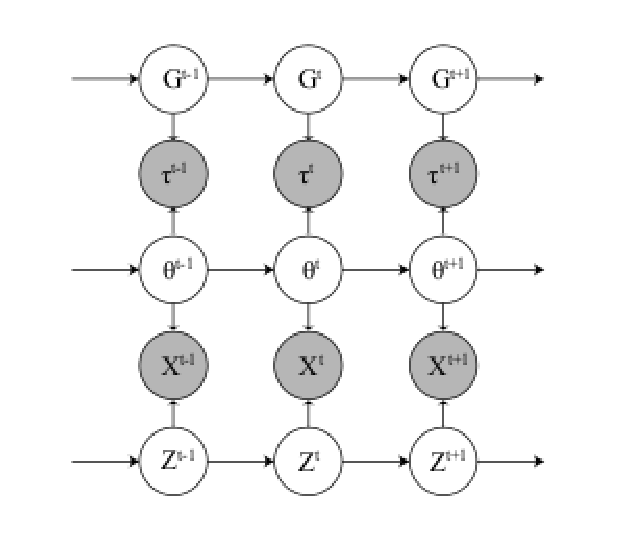
\includegraphics[width=0.5\textwidth]{ImaginiLatex/gm_mtt1.eps} 
\caption{ Graphical model describing underlying model for multi-object tracking. Shaded
nodes represent observable variables and empty nodes shows the hidden variables.
It shows overall relationship between observations $X$, $Y$, $\tau$ , camera parameters $\Theta$, ground features’ state G and targets’ states $Z$. Here, we dropped the mean-shift observation $Y$ on the graph to avoid clutter}
\end{figure}

The whole graphical showed in figure \label{ref: gm_mtt1}  is composed by the following hidden variables:
\begin{itemize}
\item \textbf{Target state} variable $Z^t = \{Z_{t,i} \}_{i=1}^{N_Z}$ containing all the information for each detected target a time $t$.The state for the target $i$ a time $t$ is composed of 6 variables $Z_ {i,t}=[ x,z,v_x,v_z,h,c]$ where:
\begin{itemize}
\item $(x, z)$ is 3D location of target in the ground plane,
\item $(v_x , v_z )$ are velocity components of target,
\item $h$ is height is target height
\item $c$ is a class indicator variable indicating the category of the target (eg. person,car)
\end{itemize}

\item \textbf{Camera state} variable $\Theta^{t}$ containing the Camera configuration parameters at time $t$. As discussed in \label{sec: Multi-Tracking Model}, the camera state is $8\times1$ vector, $\Theta_{t}=\{\phi_{\theta}, x_{\theta}, z_{\theta} f_{\theta}, u_{\theta}, v_{\theta}, h_{\theta},r_{\theta} \}$ where:
\begin{itemize}
\item $\phi_{\theta}$ is the panning angle of the camera.
\item $x_{\theta}$, $z_{\theta}$ are the 3D location respect to reference system associated to the initial frame.
\item $f_{\theta}$ is the focal length of the camera,
\item $u_{\theta}$ horizontal center point in the image plane,
\item $v_{\theta}$ horizon position  in the image plane.
\end{itemize}

\item \textbf{Ground feature state} variable $G^{t} =\{G_{t,k} \}_{k=1}^{M_G}$ for the k-Ground 3D Point. As  discussed in \ref{sec: MultiTracking Model}, the camera state is $3\times1$ vector where:
 \begin{itemize}
\item $(x, z)$ is 3D location of the ground plane;
\item $\alpha$ is a binary indicator variable encoding whether the feature is static and lies on the ground or not.
\end{itemize}
\end{itemize}
All hidden states are grouped in the Hidden Vector $\Omega^{t} = [Z_{t}, \Theta_{t}, G_{t}]$.
The observed variables in the model are features extracted on the images through object detectors and feature points detector like \textbf{KLT} or \textbf{SIFT} :
\begin{itemize}
\item \textbf{Target observation} variable $X^t =\{X_{t,j}\}_{j=1}^{N_{C}}$ containing $N_{C}$ detections provided by the object detector for the class $C=1..Nclasses$ at time $t$ stored as $5\times1$ vector $X_{t,j}= [u_c,v_c,w,p_{obj}]$ where:
\begin{itemize}
\item $(u_c,v_c)$ is the center of bounding box of the detected object,
\item $(w, h)$ are the dimensions of the bounding box,
\item $p_{obj}$ is the probability that the detected object belongs to category the class specifief by the $C$ indicator (eg. person,car).
\end{itemize}
\item \textbf{Target observation} variable $Y^t  = \{Y_{t,i} \}_{h=1}^{N}$ containing the positions in the frame $t$ at which Mean-shift tracker localize the best the matching color distribution with the i-target model.
for each tracked target variable, the tracker produces a $5\times1$ vector $Y_{t,i}= [u_c,v_c,w,s]$ where:
\begin{itemize}
\item $(u_c,v_c)$ is the location at which is centered the candidate Target,
\item $(w, h)$ are the dimensions of the bounding box,
\item $s$ is the similarity measure value between the target model and the Candidate target 
\end{itemize}
\item \textbf{Ground feature observation} $\tau_{t,k}$ containing the feature points extracted on the ground plane by applying the KLT feature detector. $\tau_{k,t}$ have two variables $(u,v)$ indicating $G_{t,k}$ location on the image plane). 
\end{itemize}
All the observations are grouped in the Visible Vector $\chi^t = [X^t , Y^t , \tau^{t}]$.

Following the optimal-filtering approach we use the probabilistic relationship between the hidden states $\Omega^{t}$ and the observations $\chi^t$ to derive the recursive equations for computing the predictive distribution $p(\Omega^{t} |\chi^{t-1})$ and the filtering distribution $p(\Omega^{t} |\chi^{t} )$ on the time step $t$ as discussed in section \ref{sec: Optimal Filtering Equations}.\\
Given the evidences $\chi^t$ and the estimates $\Omega^{t}$ at a previous time stamp, we can compute the posterior distribution $P(\Omega^{t} |\chi^t )$ as follows:

\begin{eqnarray} \label{eqn: Posterior Distribution MTT}
\underbrace{p(\Omega^{t} |\chi^{t} )}_{ \textit{posterior} } \approx  p(\chi^{t} |\Omega^{t} )
\underbrace{ \int p(\Omega^{t} | \Omega^{t-1} )p(\Omega^{t-1} |\chi^{t-1}) d\Omega^{t-1} }_{ \textit{predictive distribution} p(\Omega^{t} |\chi^{t-1}) }
\end{eqnarray}
where:
\begin{itemize}
\item $ p(\chi^{t} | \Omega^{t} )$ is the \textit{likelihood} or the \textit{Observation Model} measuring how likely are the observed data on frame $t$ given the current state estimate of hidden variables $\Omega^{t}$ ;  
\item $p(\Omega^{t} |\Omega^{t-1} )$ is the \textit{transition probability} defined by the motion model describing the dynamics of hidden variables;
\item $p(\Omega^{t-1} |\chi^{t-1} )$ is the \textit{posterior distribution} computed at previous time step $t-1$ becoming \textit{the prior distribution} at the time step $t$.
\end{itemize}

Based on the conditional independence assumption given by the formulated model, 
 the \textit{transition probabilities} can be factorized as:
\begin{eqnarray}\label{eqn: transition factorized}
p(\Omega^{t} |\Omega^{t-1} ) = 
\underbrace{p(\Theta_{t} |\Theta_{t-1} )}_{\substack{\textit{camera state} \\ \textit{dynamic model}}}
\underbrace{ p(G_t |G_{t−1}) }_{\substack{\textit{ground point} \\ \textit{dynamic model}}}
\underbrace{ p(Z_t |Z_{t−1}) }_{\substack{\textit{target state} \\ \textit{dynamic model}}}
\end{eqnarray}

Again, the \textit{likelihood} is factorized as:
\begin{eqnarray} \label{eqn: likelihood factorized}
p(\chi^{t} | \Omega^{t} )= 
\underbrace{ p(X^{t}, Y^t | \Omega^{t} )}_{\substack{\textit{detections} \\ \textit{likelihood}}}
 \underbrace{p(\tau^{t} | G^t , \Omega^{t} )}_{\substack{\textit{ground feat.} \\ \textit{point likelihood} }}
\end{eqnarray}

The final form for the posterior distribution is: 
\begin{eqnarray} \label{eqn: Posterior Distribution MTT 2}
p(\Omega^{t} |\chi^{t}) \approx \\
p(X^{t}, Y^t |\Omega^{t}) p(\tau^{t} | G^t ,\Omega^{t}) 
\int p(\Theta_{t} |\Theta_{t-1}) p(G_t |G_{t−1}) p(Z_t |Z_{t−1}) \nonumber
p(\Omega^{t-1}|\chi^{t-1}) d\Omega^{t-1}
\end{eqnarray}

In the next sections we will discuss in details how the terms in equation \ref{eqn: transition factorized} and \ref{eqn: likelihood factorized}.

\newpage

\subsection{Target Dynamic Model} 
\textbf{Target state} variable $Z^t = \{Z_{t,i} \}_{i=1}^{N_Z}$  encodes the state for the target $i$ a time $t$ as $6\times1$ variables vector $Z_ {i,t}=[ x,z,v_x,v_z,h,c]$ where:
\begin{itemize}
\item $(x, z)$ is 3D location of target in the ground plane,
\item $(v_x , v_z )$ are velocity components of target,
\item $h$ is height is target height
\item $c$ is a class indicator variable indicating the category to which belongs the target (eg. person,car)
\end{itemize}
Assuming that each Target moves independently from others we can derive a simple dynamic model for $ p(Z_t |Z_{t−1}) $, modeled as the product of the following factor:

\begin{eqnarray}\label{eqn: transition factorized}
p(Z^{t} |Z^{t-1} ) = \prod_{i=1}^{N} p(Z^{t,i} | Z^{t-1,i}) =  \\
\prod_{i=1}^{N} \underbrace{p(x_{t,i}, z_{t,i}, v_{t,i}^x,v_{t,i}^z | x_{t-1,i}, z_{t-1,i}, v_{t-1,i}^x,v_{t-1,i}^z)}_{\substack{\textit{Target motion } \\ \textit{dynamic model}}}
\underbrace{ p(h_{t,i} |h_{t-1,i})}_{\substack{\textit{Target height} \\ \textit{dynamic model}}}
\underbrace{ p(c_{t,i} |c_{t−1,i}) }_{\substack{\textit{target category} \\ \textit{dynamic model}}}
\underbrace{ p(h_{t,i} |c_{t,i}) }_{\substack{\textit{target height} \\ \textit{prior}}} \nonumber
\end{eqnarray}

where:
\begin{itemize}
\item \textit{Target motion model} encoding the dynamic of Targets in the scene, is modeled as a simple first order linear dynamic motion model with an additive gaussian noise:
$$
p(x_{t,i}, z_{t,i}, v_{t,i}^x,v_{t,i}^z | x_{t-1,i}, z_{t-1,i}, v_{t-1,i}^x,v_{t-1,i}^z)=
p(m_{t,i} | m_{t-1,i})=N(A_{4\times4} m_{t-1,i} , \Sigma_m )
$$
\item \textit{Target height dynamic model} encoding some little variation in target's height is modeled as normal distribution:
$$
p(h_{t,i} |h_{t-1,i}) =
 p(c_{t,i} |c_{t-1,i})= N(h_{t-1,i} , \sigma_h ) 
$$
\item \textit{Target category dynamic model} encoding  target's category variation in time is modeled as an indicator function since transition for category status are not allowed:
$$
 p(c_{t,i} |c_{t-1,i})= \left\{
\begin{array}{rl}
1 & \mbox{if }  c_{t,i}==c_{t-1,i} \\
0 & \mbox{otherwiswe } 
\end{array}
\right.
$$

\item \textit{Target height prior} encoding some prior information on target's height is  modeled as:
$$
 p(h_{t,i} |c_{t,i})= \left\{
\begin{array}{rcl}
 N(h_{c,i} , \sigma_{c,h} )  & \mbox{if } & c==k \\
 p_{co} & \mbox{if }  c==0  & \mbox{no object}
\end{array}
\right.
$$
\end{itemize}

In real world crowded scenes, the assumption of independently moving targets from each other is rare. Moreover, once human targets form a group, they typically tend to move together in subsequent time frames, subject to an attractive force (group model ). Again, targets rarely occupy the same physical space, so we can introduce a repulsion force to model this event. Following this considerations, we can introduce two interaction models between targets (repulsion and group model) to aid the tracking algorithm.\\
Since these two interactions are mutually exclusive, we introduce a hidden variable $\beta_{i,j,t}$ that lets us select the appropriate interaction model (mode
variable).\\
The interactions are modeled as pairwise potentials between current targets’ states, thus forming a Markov Random Field as shown on figure \ref{fig: gm_mtt2} .
\begin{figure}\label{fig: gm_mtt2}
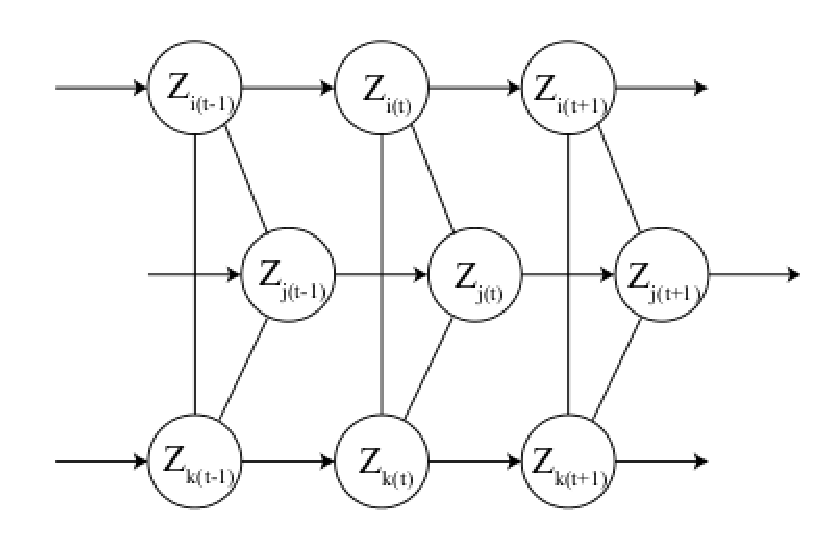
\includegraphics[width=0.5\textwidth]{ImaginiLatex/gm_mtt2.eps} 
\caption{ Graphical model describing the interaction between
targets $(i, j, k)$. The interaction is modelled by the undirected edges between   targets’ states $Z$.}
\end{figure}
Thus, the targets motion model can be farther modeled as:
\begin{eqnarray}\label{eqn: transition factorized 2}
p(Z^{t} |Z^{t-1} ) = \prod_{i=1}^{N} p(Z^{t,i} | Z^{t-1,i})= \nonumber \\
\underbrace{\prod_{i<j} \psi(Z_{i,t} , Z{j,t} |\beta_{i,j,t})}_{\substack{\textit{Interactions between} \\ \textit{Targets}}}
\underbrace{\prod_{i<j} p(\beta_{i,j,t} |\beta_{i,j,t-1} ) }_{\substack{\textit{Transition between} \\ \textit{Interactions}}}
\underbrace{\prod_{i=1}^{N} p(Z_{i,t} |Z_{i,t-1})}_{\substack{\textit{Old term} }}
\end{eqnarray}

The transition between interactions is modeled by :
$$
 p(\beta_{i,j,t} |\beta_{i,j,t-1} )= \left\{
\begin{array}{rl}
 p_{\beta}  & \mbox{if } \beta_{i,j,t} = \beta_{i,j,t-1}  \\
 1- p_{\beta} & \mbox{otherwise}
\end{array}
\right.
$$
The interactions between targets are encoded by pairwise potential able of selecting
the correct interaction model in response to the mode variable status:
$$
\psi(Z_{i,t} , Z{j,t} | \beta_{i,j,t} )= \left\{
\begin{array}{rl}
 \psi_g(Z_{i,t} , Z{j,t}) & \mbox{if} \beta_{i,j,t}=1	 \\
 \psi_r(Z_{i,t} , Z{j,t}) & \mbox{otherwise}
\end{array}
\right.
$$
The repulsion potential function  $\psi_r(Z_{i,t} , Z{j,t})$, defined so that
too close targets are pushed away, is modeled as:
\begin{eqnarray}\label{eqn: transition factorized 2}
\psi_r(Z_{i,t} , Z{j,t}) = e^{-\frac{1}{c_r r_{i,j}}}
\end{eqnarray}
where:
\begin{itemize}
\item $r_{i,j}$ denotes the distance between two targets in the 3D space;
\item $c_r$ is a parameter controlling the repulsion force between targets
\end{itemize}
This pairwise potential has larger values as two targets are located far away, and has a value closer to $0$ when two targets are nearby.

The  grouping potential function $\psi_r(Z_{i,t} , Z{j,t})$  is defined with the assumption that grouped targets move together, keeping the same distance (group movement), and the same relative location in consecutive time frames as well. This assumption can be modeled as $p_{i,t} − p_{j,t} \approx p_{i,t-1} - p_{j,t-1}$, which is in turn equivalent to $v_{i,t} \approx v_{j,t}$ , where $p_{i,t}$ is the target’s location in 3D and $v_{i,t}$ is the velocity component of $Z_{i,t}$ .
Thus, we model the group motion potential as:
\begin{eqnarray} \label{eqn: group motion potential}
\psi_g(Z_{i,t} , Z{j,t}) = \frac{1}{e^{s_g(r_{i,j}-tg)} } e^{-c_g \| v_{t,i}-v_{t,j} \|} 
\end{eqnarray}
where:
\begin{itemize}
\item $s_g$ is the parameter controlling the slope of soft step function
used to enforce that the distance $r_{i,j}$ between two targets should be close enough in order to be considered as a group;
\item $t_g$ is a distance threshold for the soft function;
\item $c_g$ is a parameter controlling the similarity of velocities.
\end{itemize}
This pairwise potential has larger values as two near targets moves with same velocity, and has a value closer to $0$ when two targets are are located far away or moves with different velocities.


\section{Camera Motion Model}
In order to deal with camera motion, we also model camera motion parameters. Note that the camera parameters are coupled with the target and feature observations and cannot be directly observed.  
\textbf{Camera state} $\Theta^{t}$ is the variable containing the Camera configuration parameters at time $t$. As discussed in \ref{sec: MultiTracking Model}, the camera state is $8\times1$ vector, $\Theta_{t}=\{\phi_{\theta}, x_{\theta}, z_{\theta}, f_{\theta}, u_{\theta}, v_{\theta}, h_{\theta},r_{\theta} \}$ where:
\begin{itemize}
\item $\phi_{\theta}$ is the panning angle of the camera;
\item $x_{\theta}$, $z_{\theta}$ are the 3D location respect to reference system associated to the initial frame;
\item $f_{\theta}$ is the focal length of the camera;
\item $u_{\theta}$ is horizontal center point in the image plane;
\item $v_{\theta}$ is horizon position  in the image plane;
\item $r_{\theta}$ is the absolute velocity of camera.
\end{itemize}
The temporal relationship between camera position is simply represented as a linear dynamic model:
\begin{eqnarray} \label{eqn: camera dynamics}
x_{t,\theta} = x_{t-1,\theta} - r_{t-1,\theta} \sin(\phi_{t-1,\theta} )dt \\
z_{t,\theta} = z_{t-1,\theta} + r_{t-1,\theta} \cos(\phi_{t-1,\theta} )dt
\end{eqnarray}
We defined the positive value of $\phi$ for the left direction so there appears minus
sign on $x_t$.\\
The uncertainty on the other camera parameters $( f_{\theta}, u_{\theta}, v_{\theta}, h_{\theta}, \phi_{\theta})$ is just modeled with additive gaussian noise. The final motion model for the camera model is given by
\begin{eqnarray} \label{eqn: camera dynamics}
p(\Theta_{t} |\Theta_{t-1} )= 
 \left[
\begin{array}{c}
x_{t,\theta}  \\
z_{t,\theta}  \\
f_{t,\theta} \\
u_{t,\theta} \\
v_{t,\theta} \\
h_{t,\theta} \\
\phi_{t,\theta} \\
r_{t,\theta}
\end{array}
\right]
=
N(\left[
\begin{array}{c}
x_{t-1,\theta} - r_{t-1,\theta} \sin(\phi_{t-1,\theta} )dt \\
z_{t-1,\theta} + r_{t-1,\theta} \cos(\phi_{t-1,\theta} )dt \\
f_{t-1,\theta} \\
u_{t-1,\theta} \\
v_{t-1,\theta} \\
h_{t-1,\theta} \\
\phi_{t-1,\theta} \\
r_{t-1,\theta}
\end{array}
\right], W)
\end{eqnarray}
where $W$ is $8\times8$ diagonal matrix containing gaussian noise covariance.

\section{Ground feature Dynamic Model}
As stated in \ref{sec: MultiTracking Model} we use KLT tracker to track
stationary features on the ground so as to get a robust estimate of the camera
motion. This is achieved by introducing the hidden state $G_{i,t}$ which captures
the true location of a ground feature in 3D.
As  discussed in \ref{sec: MultiTracking Model}, the ground point state is $3\times1$ vector where:
 \begin{itemize}
\item $(x, z)$ is 3D location of the ground plane;
\item $\alpha$ is a binary indicator variable encoding whether the feature is static and lies on the ground or not.
\end{itemize} 
Let $\tau{i,t}$ be the ground feature tracked in the image plane at time $t$, and $\hat{\tau{i,t}}$ the projection of $G_{i,t}$ into the image plane at time $t$. This indicates the expected location of the feature $G_{i,t}$ at t. Clearly we are interested only on location of  $\tau{i,t}$ and $\hat{\tau{i,t}}$ in image plane.
Assuming the ground plane features are static, the motion model of  $G_{i,t}$ will have a simple form of indicator function:

\begin{eqnarray} \label{eqn: Ground dynamics}
 p(G_{t,i} |G_{t-1,i})= \left\{
\begin{array}{rl}
1 & \mbox{if }  G_{t,i}==G_{t-1,i} \\
0 & \mbox{otherwiswe } 
\end{array}
\right.
\end{eqnarray}

\section{Observations likelihood}
As, discussed in section \ref{eqn: likelihood factorized} the observation \textit{likelihood} is factorized as product of $2$ independent components:
the target detections likelihood $p(X^{t}, Y^t | \Omega^{t})$ and the ground point likelihood $p(\tau^{t} | G^t , \Omega^{t})$.\\
The observations likelihood  $p(X^t, Y^t |Z^t, \Theta^t)$ between the target states $Z^t$ and observation $\{X^t, Y^t \}$ is factorized as the product of two independent normal distribution depending on camera projection function $f_P$:
\begin{eqnarray} \label{eqn: observations likelihood}
p(X^t,Y^t | Z^t , \Theta^t )= p(X^t | Z^t , \Theta^t )p( Y^t | Z^t , \Theta^t ) = \\ \nonumber
N(f_P(Z_{i,t}),W) N(f_P(Z_{i,t}),V)
\end{eqnarray}
The relationship $p(\tau^t |G^t , \Theta^t )$ between the ground point state $G^t$ and observation $\tau^t$,  can be modeled using the camera projection function$ f_P$ if the feature is truely static and lying on the ground plane ($\alpha=1$). \\
However, if either the feature is moving or the feature is not on the ground plane ($\alpha=0$), the projection function $f_P$ does not model the correct relationship between $\tau_{t,i}$ and $G_{t,i}$ . 
Thus, the observation process is modeled as:
\begin{eqnarray} \label{eqn: Ground observation Model}
p(\tau^t | G^t , \Theta^t ) \approx
\left\{
\begin{array}{rl}
 N(f_P (G_{t,i} , Θt ), \Sigma_G ) & \mbox{if }  \alpha_i==1 \\
 unif (p_G )  & \mbox{otherwise }
\end{array}
 \right.
\end{eqnarray}
Similar to the class variable in target model, those features that are not consistent with the majority of other features will be automatically filtered out.

\newpage
\section{Maximum aposterior solution by MCMC Particle Filter}
Considering the complexity of the given probabilistic formulation, it is extremely challenging to design an analytical inference method for estimating the Maximum aposterior solution. This challenge is due to the presence of the high nonlinearity of projection function, the MRF induced by pairwise potential and the non-gaussian nature of the posterior and prior distribution. 
Instead of relying on an analytical solution, we employ a sampling based sequential filtering technique based on the Monte-Carlo Markov-Chain (\textbf{MCMC Particle Filter})
Using \textbf{MCMC} sampling scheme we can propagate samples without weights in the particle filtering framework to get an approximation of the final posterior distribution .
Specifically, at each time step $t$ given a set of $N$ prediction on hidden variable status $\Omega^{t-1}$  we can approximate the prior distribution:
\begin{eqnarray} \label{eqn: Predictive Approximation}
p(\Omega^{t-1} |\chi^{t-1}) \approx \{ \Omega_r^{t-1} \}_{r=1}^N
\end{eqnarray}
Propagating this samples in the \textit{Motion Model} we generate samples for the \textit{Predictive Distribution} and are able to approximate the integral in \ref{eqn: Posterior Distribution MTT 2} via Monte Carlo integration:\\
\begin{eqnarray} \label{eqn: MonteCarlo Approx. Predictive}	
\int p(\Theta_{t} |\Theta_{t-1}) p(G_t |G_{t−1}) p(Z_t |Z_{t−1})p(\Omega^{t-1}|\chi^{t-1}) d\Omega^{t-1} \approx \\ \nonumber
\sum_{r=1}^{N} p(\Theta^{t} | \Theta^{t-1}_r) p(G_t |G^{t-1}_r) p(Z^t |Z^{t-1}_r) 
\end{eqnarray}
Subsequently the final posterior distribution in time $t$ can be approximated by following equation:
\begin{eqnarray} \label{eqn: Posterior Distribution MTT3}
p(\Omega^{t} |\chi^{t}) \approx  p(X^{t}, Y^t |\Omega^{t}) p(\tau^{t} | G^t ,\Omega^{t}) 
\sum_{r=1}^{N} p(\Theta^{t} | \Theta^{t-1}_r) p(G_t |G^{t-1}_r) p(Z^t |Z^{t-1}_r)
\end{eqnarray}
This distribution will be the target distribution of our markov chain montecarlo method.
Once the sampling method has reached convergency we are able to derivate the Maximum aposterior estimate for $\Omega^{t}$ simply by choosing the sample with maximum a posteriori probability value: \\
\[
 \operatorname{arg\,max}_{\Omega^{t}} p(X^{t}, Y^t |\Theta^{t}) p(\tau^{t} | G^t ,\Omega^{t}) p(\Theta^{t} |\chi^{t-1}) 
\]
As a condition for the construction of an MCMC method, we need to design a Markov chain over the joint space of $\Omega$. 
This has the same stationary distribution as the posterior distribution 
$p(\Omega^{t-1} |\chi^{t-1})$. 
We define a \textit{proposal distribution} as able of generating:
\begin{itemize}
\item samples for all existing targets, features and camera variable. 
\item appropriate random perturbation to the chosen node additive gaussian or switching state.
\end{itemize}
The proposal density can be generated with the following steps: 
\\
\\
{\bf PROPOSAL DISTRIBUTION GENERATION}\\[.4cm]
{\sf
0. \hspace*{0.2cm} At each time $t$, choose randomly one hidden state variable camera  $\Theta^t$,\\
\hspace*{0.9cm} target $Z_i^t$ or feature $G_i^t$ with a probability
$$
  p_i=\frac{w_i}{\sum_{k=0}^{M} w_k}
$$
1.  \hspace*{0.2cm} if(Sampled State Variable is Camera $\Theta^t$) \\
1.1 \hspace*{0.4cm} generate $\Theta^r=N(\Theta^{t-1},S_{\Theta})$\\
\\
2.  \hspace*{0.2cm} if(Sampled Variable is the $i$-Target $Z_i^t=\{x_i, z_i, v_i^x , v_i^z , h_i,c_i \}_i$) \\ 
2.1 \hspace*{0.4cm} generate $Z_i^r=\{x_i, z_i, v_i^x , v_i^z , h_i \}$ from $N(Z_i^{t-1},S_{Z}^t)$ \\
2.2 \hspace*{0.4cm} set the class variable $c_i$ by switching randomly $c_i^{t-1}$, with a probability \\ 
\hspace*{0.9cm} of switching $p_{c}^f$ \\
2.3 \hspace*{0.4cm} set $\beta_{i,j}^t$ for all $j$ by switching randomly interaction mode $\beta_{i,j}^{t-1}$, \\ 
\hspace*{0.9cm}  with a probability of switching $p_{\beta}$ \\
\\
3.  \hspace*{0.2cm} if(Sampled Variable is the $j$-Ground point $G_j=\{x_j, z_j\}$ \\
3.1 \hspace*{0.4cm} generate $G_j^r=N(G_j^{t-1},S_G^t)$ \\
3.2 \hspace*{0.4cm} set the indicator variable $\alpha_j^t$ by switching randomly $\alpha_j^t$,\\
\hspace*{0.9cm}  with a probability of switching $p_{\alpha}^f$ 
}\\[.4cm]
\\
\\
Assigning high weight values $w_i$ to the camera's state variable we are able to generate an larger number of samples respect with the others variables. In this way we can capute camera's variability making more robust the whole estimation process since camera parameters are coupled with all states giving more sensitivity of results to the camera estimated status.\\

\newpage
\section{The Algorithm}
The Complete procedure for the Sequential Bayesian Estimation of  at each time step $t$ can be summarized in the following  main steps:
\\
{\bf MCMC MULTIPLE TRACKING }\\[.4cm]
{\sf
\textbf{INPUT:}\\
[.2cm] \textbf{ Observed variable} $\chi^t$ on current image $I_t$:\\
 \hspace*{0.2cm} \textit{Target detections} $X^t=\{X_{t,i}\}_{i=1}^{X^{detections}}={[u_i,v_i,h_i,w_i,p_i]^t}_{i=1...X^{ detections}}$ \\
 \hspace*{0.2cm} \textit{Target detections} $Y^t =\{Y_{t,j}\}_{j=1...Y^{ detections}}={[u_j,v_j,h_d,w_j,p_j]^t}_{j=1...Y^{detections}}$\\
 \hspace*{0.2cm} \textit{Ground point detections} $\tau^t =\{\tau_{t,g}\}_{g=1...\tau^{ detections}}={[u_h,v_h]^t}_{g=1...\tau^{detections}}$
\\
\\
[.2cm] \textbf{ Hidden states} $\Omega^{t-1}$ on previous time $t-1$\\
 \hspace*{0.2cm} \textit{Target state} $Z^{t-1} = \{Z_{{t-1},k} \}_{k=1}^{NZ_{t-1}}=[ x_k,z_i,v_k^x,v_k^z,h_k,c_k]_{k=1..NZ_{t-1}}^{t-1}$\\
 \hspace*{0.2cm} \textit{Camera state} variable $\Theta^{t-1}=[\phi_{\theta}, x_{\theta}, z_{\theta} f_{\theta}, u_{\theta}, v_{\theta}, h_{\theta},r_{\theta}]^{t-1}$\\
 \hspace*{0.2cm} \textit{Ground feature state} variable $G^{t-1} =\{G_{(t-1),l} \}_{l=1}^{NG}=[x_l,z_l,\alpha_l]_{k=1..NG}^{t-1}$
\\
\\
\textbf{OUTPUT:}\\ 
[.2cm] \textbf{ Maximum aposterior estimate} on current time $t$, $\Omega^{t}=\{Z^{t},\Theta^{t},G^{t}\}$\\
%[.4cm] \textbf{Target state} $Z^{t}$\\
%[.4cm] \textbf{Camera state} $\Theta^{t-1}$\\
%[.4cm]\textbf{Ground feature state} $G^{t-1}$\\
\\
0. Solve the \textit{Association Problem} to find correspondences between detected Targets on image at current time $Det=\{(X_{t,i}, Y_{t,i})):X_{t,i} \in X^t,Y_{t,i} \in Y^t\}$ and the Target State Variables $Z^{t}$ at current time.\\
A subset  of $Det$ will be associated to $Z^t$.\\ 
\\
1. Calculate \textit{Montecarlo approximation} of the predictive distribution:\\
$$
 p(\Omega^{t} |\chi^{t-1}) \approx \\ \nonumber
\sum_{r=1}^{N} p(\Theta^{t} | \Theta^{t-1}_r) p(G_t |G^{t-1}_r) p(Z^t |Z^{t-1}_r) 
$$
\\
\\
2. \textit{Sampling generation} for $p(\Omega^{t} |\chi^{t})$ via MCMC sampling scheme:\\
$$
p(\Omega^{t} |\chi^{t}) \approx  p(X^{t}, Y^t |\Omega^{t}) p(\tau^{t} | G^t ,\Omega^{t}) 
p(\Omega^{t} |\chi^{t-1})
$$
\\
3. Find \textit{Maximum aposterior} estimate $\Omega^{t}$ for $p(\Omega^{t} |\chi^{t})$:\\
\[
 \operatorname{arg\,max}_{\Omega^{t}} p(X^{t}, Y^t |\Theta^{t}) p(\tau^{t} | G^t ,\Omega^{t}) p(\Theta^{t} |\chi^{t-1}) 
\]
}\\[.4cm]
\\
\\

